\documentclass[11pt,twoside]{article}

\usepackage{paperlighter}

% Recommended, but optional, packages for figures and better typesetting:
\usepackage{microtype}
\usepackage{graphicx}
\usepackage{subfigure}
\usepackage{booktabs} % for professional tables

% Attempt to make hyperref and algorithmic work together better:
\newcommand{\theHalgorithm}{\arabic{algorithm}}


% For theorems and such
\usepackage{amsmath}
\usepackage{amssymb}
\usepackage{mathtools}
\usepackage{amsthm}

% if you use cleveref..
\usepackage[capitalize,noabbrev]{cleveref}

%%%%%%%%%%%%%%%%%%%%%%%%%%%%%%%%
% THEOREMS
%%%%%%%%%%%%%%%%%%%%%%%%%%%%%%%%
\theoremstyle{plain}
\newtheorem{theorem}{Theorem}[section]
\newtheorem{proposition}[theorem]{Proposition}
\newtheorem{lemma}[theorem]{Lemma}
\newtheorem{corollary}[theorem]{Corollary}
\theoremstyle{definition}
\newtheorem{definition}[theorem]{Definition}
\newtheorem{assumption}[theorem]{Assumption}
\theoremstyle{remark}
\newtheorem{remark}[theorem]{Remark}

% Todonotes is useful during development; simply uncomment the next line
%    and comment out the line below the next line to turn off comments
%\usepackage[disable,textsize=tiny]{todonotes}
\usepackage[textsize=tiny]{todonotes}



\slimtitle{Bayesian deep learning}
\slimauthor{DURAND Enzo & DAM Damien}


\begin{document}

\lightertitle{Bayesian deep learning}

\lighterauthor{DURAND Enzo$^{\dagger}$, DAM Damien$^{\ddagger}$}

\vspace{1cm}
\begin{abstract}

The goal of this practical work is to understand the different types of transfer learning with a focus on computer vision. Some tools such as saliency maps can also help us understand the inside of neural networks. Thanks to these we can see how adversarial attacks work in computer vision. After that we worked on domain adaptation and generative adversarial networks.

\end{abstract}

% \begin{figure}[H]
% \begin{tabular}{cc}
% \subfloat{\includegraphics[width=8cm]{img/acc_lr.png}} &
% \subfloat{\includegraphics[width=8cm]{img/loss_lr.png}}
% \end{tabular}
% \end{figure}

\section{Linear regression}

1.2) We can see that, the more the data, the more the certainty of the results. The posterior distribution becomes way less uncertain when adding data points.

\begin{figure}[H]
  \centering
    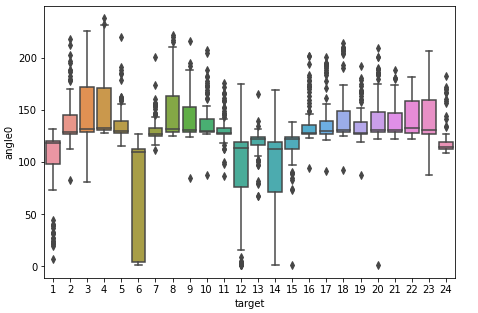
\includegraphics[width=15cm]{img/1.png}
\end{figure}

1.5) When alpha is equal to 0, we don't use the prior over the parameters anymore and only the second term of the equation is remaining. The second term gives us a hint about the uncertainty over the parameters. The uncertainty is large when there is not much data available as noticed in the first question, that's why the uncertainty increases when far from the training distribution.

\begin{figure}[H]
  \centering
    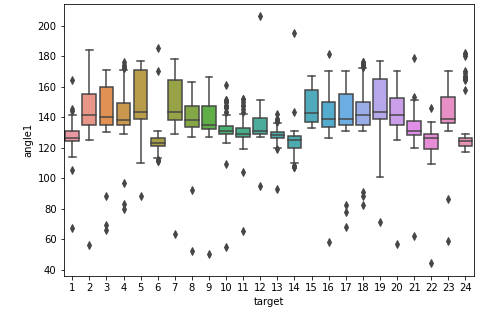
\includegraphics[width=15cm]{img/2.png}
\end{figure}
 
1.5b) The model still outputs nice results on that new dataset. There is a lower variance and low uncertainty, probably because the training points are really close to ground truth.

\begin{figure}[H]
  \centering
    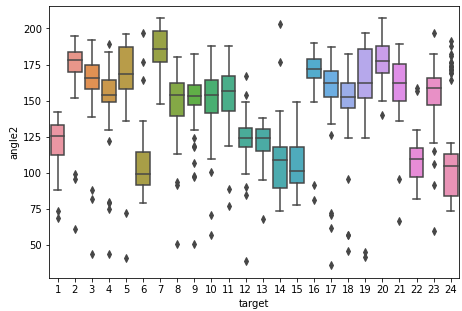
\includegraphics[width=15cm]{img/3.png}
\end{figure}

2.2) Here we can see that the variance is very large out of the training area but almost null in training area. We can explain that by the fact that the data points only represent a small part of the ground truth distribution.

\begin{figure}[H]
  \centering
    \includegraphics[width=15cm]{img/4.png}
\end{figure}

2.4) Now the variance is close to zero even out of the training area. We can explain it by the fact that the gaussian basis function is more local and not really efficient when going away from the training points.

\begin{figure}[H]
  \centering
    \includegraphics[width=15cm]{img/5.png}
\end{figure}

2.5) When using localized basis functions, the data points are important for a certain region of the space. Whereas in other regions of the space, the heteroscedastic uncertainty is zero so the homoscedastic uncertainty is equal to the inverse of beta which is 0.08 (1/12).

\section{Approximate inference}

1.1) The model confidence seems to be the same around and far from the training distribution. This is because it is doing a MAP estimation, which isn't taking in account uncertainty over w.

\begin{figure}[H]
  \centering
    \includegraphics[width=8cm]{img/6.png}
\end{figure}

1.2) We are no longer doing a MAP estimation because here the predictive distribution is computed using the parameters sampled from the estimated posterior distribution. Uncertainty is now taken into account, which explains why we can see uncertainty far from the training distribution.

\begin{figure}[H]
\centering
\includegraphics[width=8cm]{img/7.png}
\end{figure}

1.3) We are now using variational inference, which takes into account uncertainty over the parameters by approximating its posterior distribution through the use of ELBO. This is achieved by sampling using MC, in contrast to MAP estimation. This leads to uncertainty that is far from the data distribution, as is the case with Laplace approximation.

\begin{figure}[H]
\centering
\includegraphics[width=8cm]{img/8.png}
\end{figure}

2.1) In this figure, we can see the classification analysis for the variational model with and without dropout. We observe that both models achieve a perfect accuracy on the training data. The difference lies in the uncertainty of the models: the one with dropout seems to have a more complex modeling of uncertainty, and it would probably perform better on test data. Inconsistencies are due to the randomness introduced by dropout.

\begin{figure}[H]
\begin{tabular}{cc}
\subfloat{\includegraphics[width=8cm]{img/9.png}} &
\subfloat{\includegraphics[width=8cm]{img/10.png}}
\end{tabular}
\end{figure}

\section{Applications of Uncertainty}

1.1) In the images that are difficult to classify, such as the third one, there are many different bars in the mean probabilities, which indicates that the model struggles to make a choice. The max probability frequency bar graph can be interpreted in the same way. The last three columns provide insight into the most probable classes. For the third image, we can see that the model hesitates between 3, 5, and 2, which seems fair even to the human eye. Conversely, for the second image, which is obviously a 5, the columns are much cleaner. The network has total confidence in its prediction, with 100\% mean probabilities for the 5 class. The last three columns show that the 9 and 7 classes have 0\% probability, which is consistent with the network's confidence.

\begin{figure}[H]
\centering
\includegraphics[width=15cm]{img/11.png}
\end{figure}

\begin{figure}[H]
\centering
\includegraphics[width=15cm]{img/12.png}
\end{figure}

2.1) The goal here is to detect failures, and upon examining the graph, we can see that ConfidNet has the highest AUPR, followed by MCDropout and then MCP. This means that ConfidNet is the best at this task. We chose AUPR instead of AUROC because the ratio of wrong predictions to correct predictions might be highly unbalanced.

\begin{figure}[H]
\centering
\includegraphics[width=8cm]{img/13.png}
\end{figure}

3.1) Here, the goal is to detect out-of-distribution examples. Upon inspection of the graph, it can be seen that ODIN performs slightly better than MCDropout, with MCP being the last. These results seem legitimate because ODIN is built on top of MCP, resulting in better performance. ODIN is the best model here because its inverse adversarial attack process enhances the softmax of in-distribution inputs, making it more separable from out-of-distribution examples.

\begin{figure}[H]
  \centering
    \includegraphics[width=8cm]{img/14.png}
\end{figure}

\end{document}